\chapter[Topic Definition]{Topic Definition}
\label{Chap:label}	%CREATE YOUR OWN LABEL.
\pagestyle{headings}


\section{Topic}





While no single solution can completely safeguard an edge network, an effective approach to mitigating unauthorised/unwanted network 
traffic is by simply filtering out potentially malicious packets. The proposed thesis project aims to alleviate some of these potential security issues by 
designing a customised FPGA packet filter featuring a customised Etherent MAC and web server on a RISC-V processor.  By accelerating the filtering in hardware, 
new levels of parallelism, latency and efficiency can be gained compared to current software based implementations. 

The packet filter will selectively filter based on various 
criteria that can be configured through a customised web interface running on the RISC-V softcore processor. This web interface will also display real-time metrics enabling users to monitor network activity. This project will have potentially significant practical applications in the field of edge network security offering an efficient and cost-effective solution alternative to current options in the market.


\section{System Overview}
\subsection{Hardware Overview}

The proposed system consists of two inputs and outputs, namely two ethernet interfaces which can be seen in figure \ref{fig:sys-overview}. This project uses the 
Xilinx Artix 7 XC7A100T FPGA and two LAN8720A RMII interface chips. The Interface on the left of figure \ref{fig:sys-overview} is where the internal/private 
network is attached. The right Ethernet interface is where the external/public network connects. 

\begin{figure}[h]
    \centering
    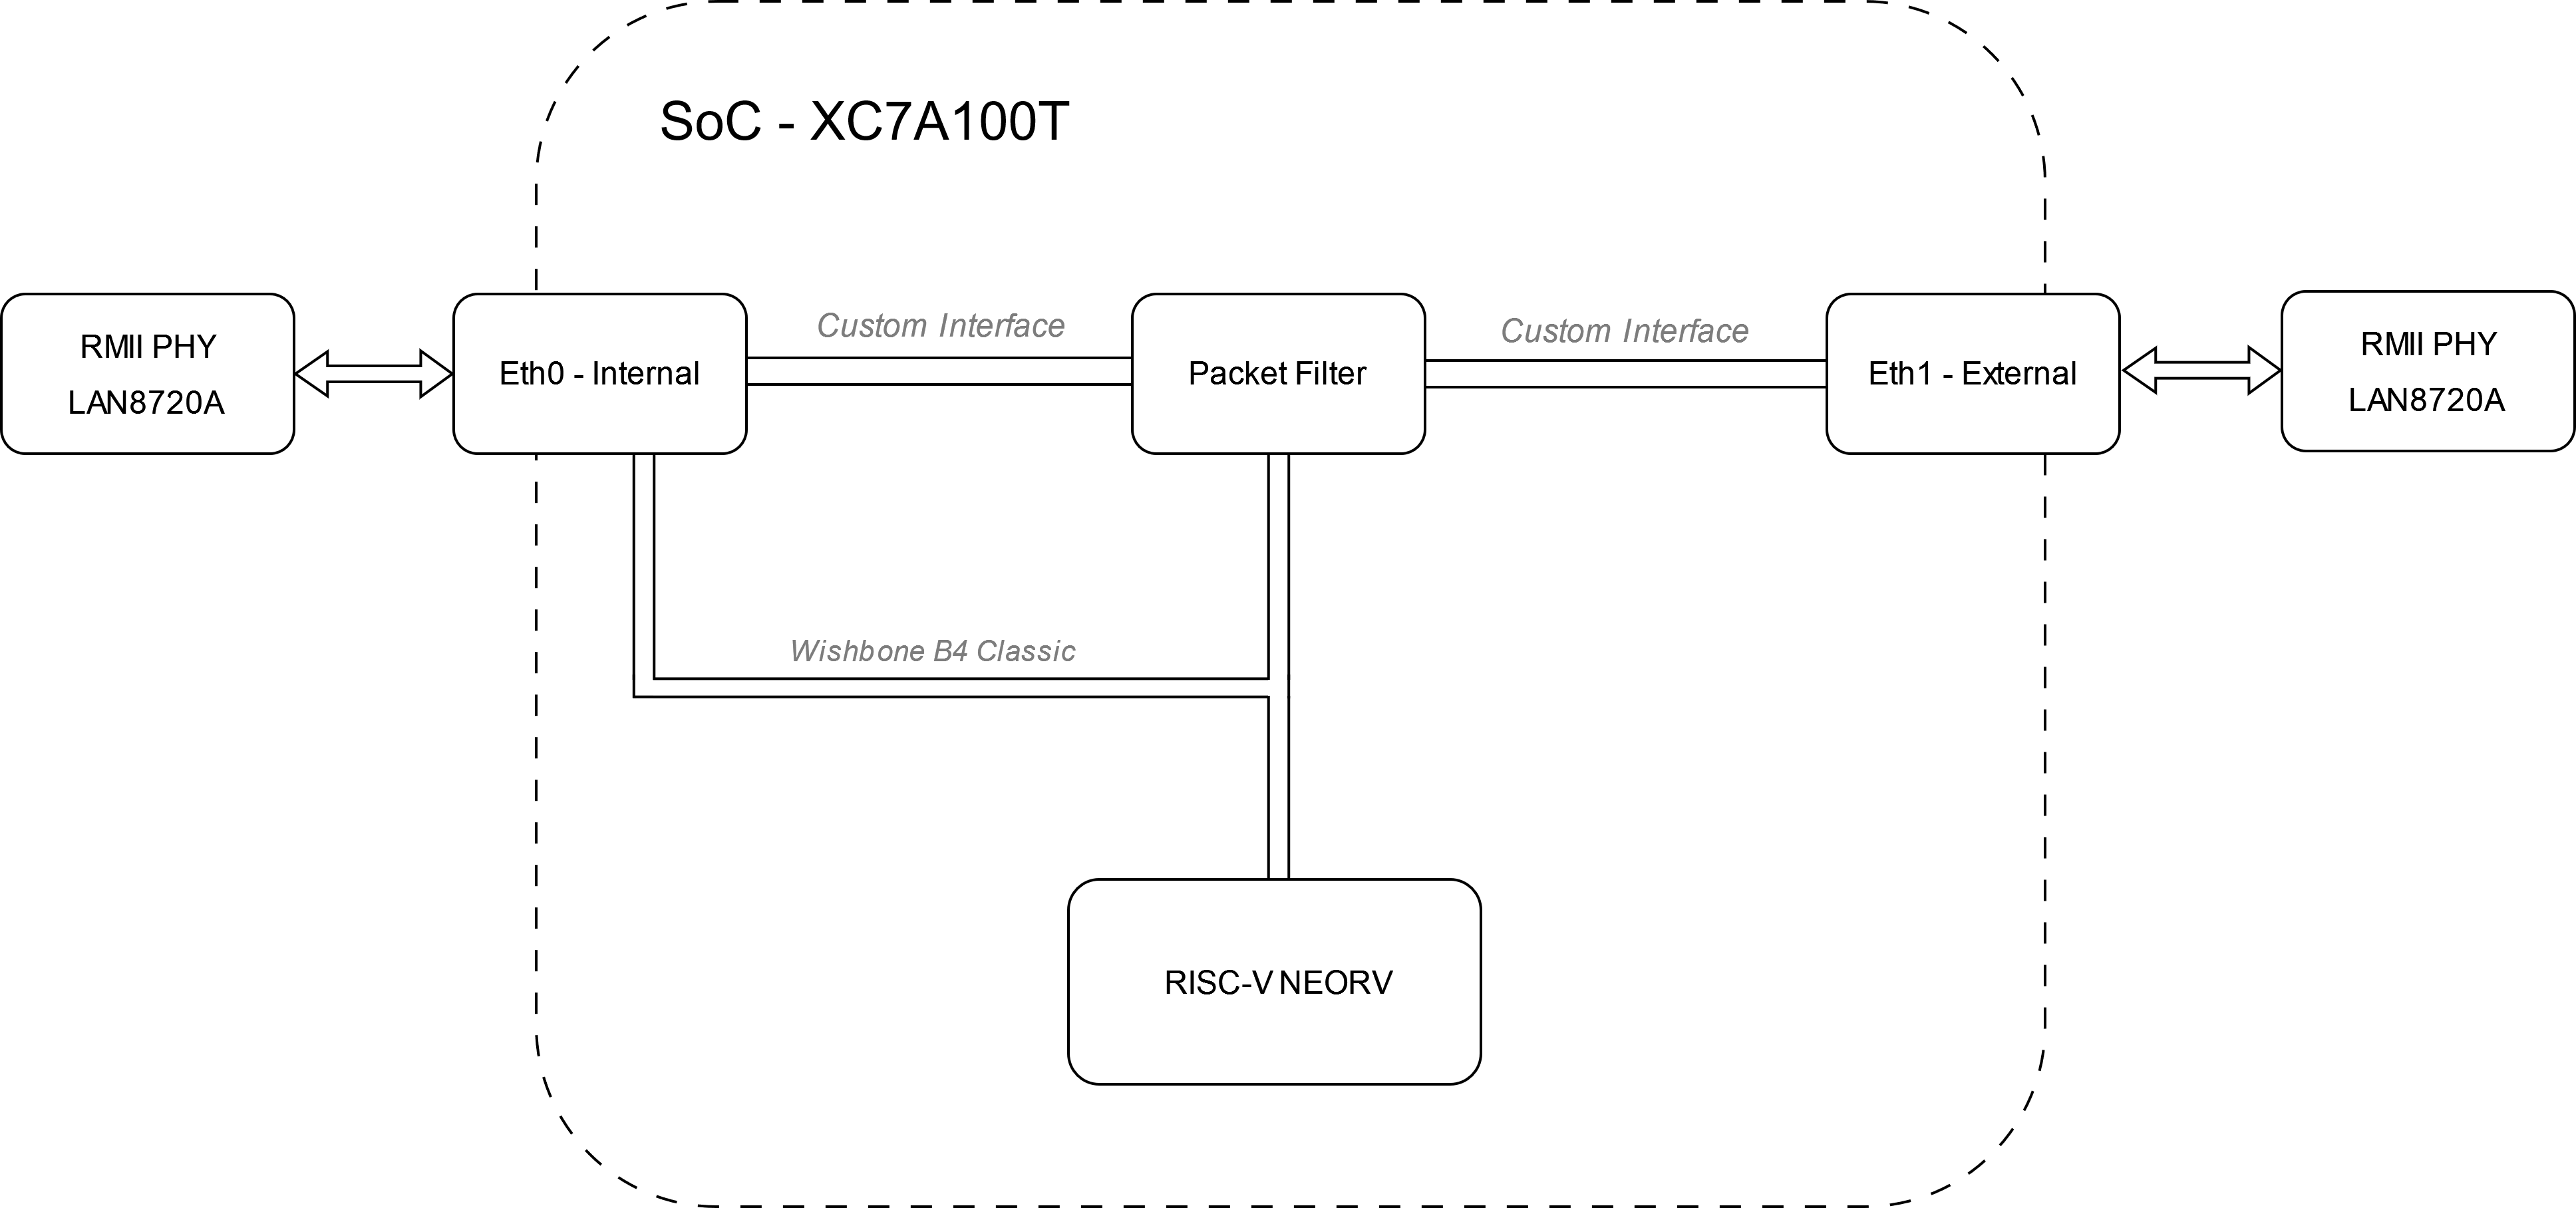
\includegraphics[width=1\textwidth]{Images/ThesisSystemsOverview.png}
    \caption{System overview}
    \label{fig:sys-overview}
\end{figure}

\newpage

The hardware packet filter will be connected along with the two Ethernet PHY interfaces to the RISC-V softcore processor using the Wishbone B4 classic interface. 
The two Ethernet PHYs will be connected through the packet filter using a custom high speed interface to reduce the dependance of the microprocessor in the 
filtering of IP packets. 

\subsubsection{Implications}

Only the internal Ethernet interface is connected to the microprocessor which limits the web page access to devices on the private network. This is proposed to 
increase the security and only allow configuration of the packet filter from a computer within the protected network.

\subsection{Packet filtering hardware algorithms}
As of this project proposal, a classification algorithm has not been decided on. Several designs are under consideration including both a new customised design and the one proposed 
in \cite{FastRecongifFPGAFirewall}.


\subsection{Microprocessor selection}
The proposed project will use the NEORV32\footnote[1]{See: https://github.com/stnolting/neorv32} RISC-V softcore microprocessor. This microprocessor will  
run FreeRTOS with the FreeRTOS-Plus-TCP network stack to handle the control of the packet filter and host a web server. Additional libraries such as the 
FreeRTOS-Plus-FAT will also be used to store web content such as HTML files. 



\section{Aims}

The aims of the proposed FPGA Ethernet controller and web interface on a RISC-V processor are:

\begin{itemize}
    \item Increase security to edge IoT networks,
    \item Increase the power efficiency for wire-speed firewalls, and
    \item Decrease the latency for packet filter firewalls.
\end{itemize}



\section{Establishing Exclusions}

While the proposed project will reduce the likelihood of network based attacks it is not a \textit{'one size fits all'} solution. 
By the nature of the IoT and edge network ecosystem, there are a myriad of different attack vectors where not all of them will be detectable at the
network level.

The proposed project will \textbf{not}
\begin{itemize}
    \item Protect against all attacks,
    \item Be able to protect against all IoT devices,
    \item Perform routing,
    \item IPv6 Packets, or
    \item Perform network address translation (NAT)
\end{itemize}



\section{Performance Indicators}
The key performance indicators gauge a level of success for the project and are as follows: 

\begin{itemize}
    \item Throughput at which the packet filter can work,
    \item Added latency to the network,
    \item Resource utilisation (low look-up table and flip flop count) to fit on an Artix 7-100T FPGA,
    \item Web server access on a remote machine, and
    \item Web server concurrency - multiple connections
\end{itemize}



\section{Required Equipment}
While the hardware design will be developed in such a way that it is vendor-agnostic, to test the design a Digilent Nexys A7-100T development board will be used.
Importantly, this board has a RJ45 connector and LAN8720 RMII interface chip which allows for a regular Fast Ethernet connection to be directly connected 
to the FPGA board. An additional LAN8720 ETH board from Waveshare is also required to obtain the secondary interface. 

To validate the functionality and effectiveness of the design, it will be compared with a Raspberry Pi Compute Module 4 (CM4) with a Waveshare CM4-DUAL-ETH-MINI 
daughterboard which contains two 1GbE interfaces. This will act as a baseline. A summary of the required items can be seen below.

\begin{itemize}
    \item Digilent Nexys A7 100T FPGA board,
    \item Waveshare LAN8720A ETH Board,
    \item Waveshare CM4-DUAL-ETH-MINI Router board,
    \item Raspberry Pi Compute Module 4,
    \item 32GB MicroSD card,
    \item USB Power supply,
    \item An assortment of Cat 5e or better Ethernet cables
    \item Target/Victim and Attacking Computers
\end{itemize}


\section{Technology Readiness Level}

One method for estimating the degree of maturity for a technical project is by using the \textit{Technology Readiness Levels (TRL)} benchmark. Within this, 
there are 9 levels each indicating a different phases of a design. This project is intended to reach a TRL of 6. These six different levels and their 
relevance to this project are as follows. 

\begin{enumerate}
    \item \textbf{TRL 1: Basic Research} - The concepts are researched and a base understanding of the system is gathered,
    \item \textbf{TRL 2: Applied Research} - Detailed research is conducted into each part of the project,
    \item \textbf{TRL 3: Proof of Concept} - A cutdown version of the final project protoype that highlights the core functionality or subsystems working,
    \item \textbf{TRL 4: Lab Testing of Prototype} - Prototype of the core design with majority of the functionality working,
    \item \textbf{TRL 5: Testing of Integrated system} - Refined prototype that works as intended but may be incomplete, and
    \item \textbf{TRL 6: Prototype System Verified} - Comparison to pre-existing solutions and verification. 
\end{enumerate}


